\utsubsection{Handover-Modul}{Stefan Giggenbach}\label{sec:hom}

Das implementierte Handover-Modul muss im Prinzip die am Ende des Abschnitts \ref{sec:handover} beschriebenen Aufgaben abarbeiten. Die Erfassung der Measurement Reports wurde bereits in Abschnitt \ref{sec:measrep} beschrieben. Dabei wird, wie bereits erwähnt, nicht die vorhandene SQLite3-Datenbank, sondern zwei neu erstellte Klassen, deren Klassendiagramme in Abbildung \ref{fig:homclass} dargestellt sind, verwendet. Die Definition und Implementierung befindet sich in den Dateien \lstinline{GSMHandover.h} und \lstinline{GSMHandover.cpp} des \textit{GSM}-Moduls.

\begin{figure}[h!t!b!p!]
  \centering
  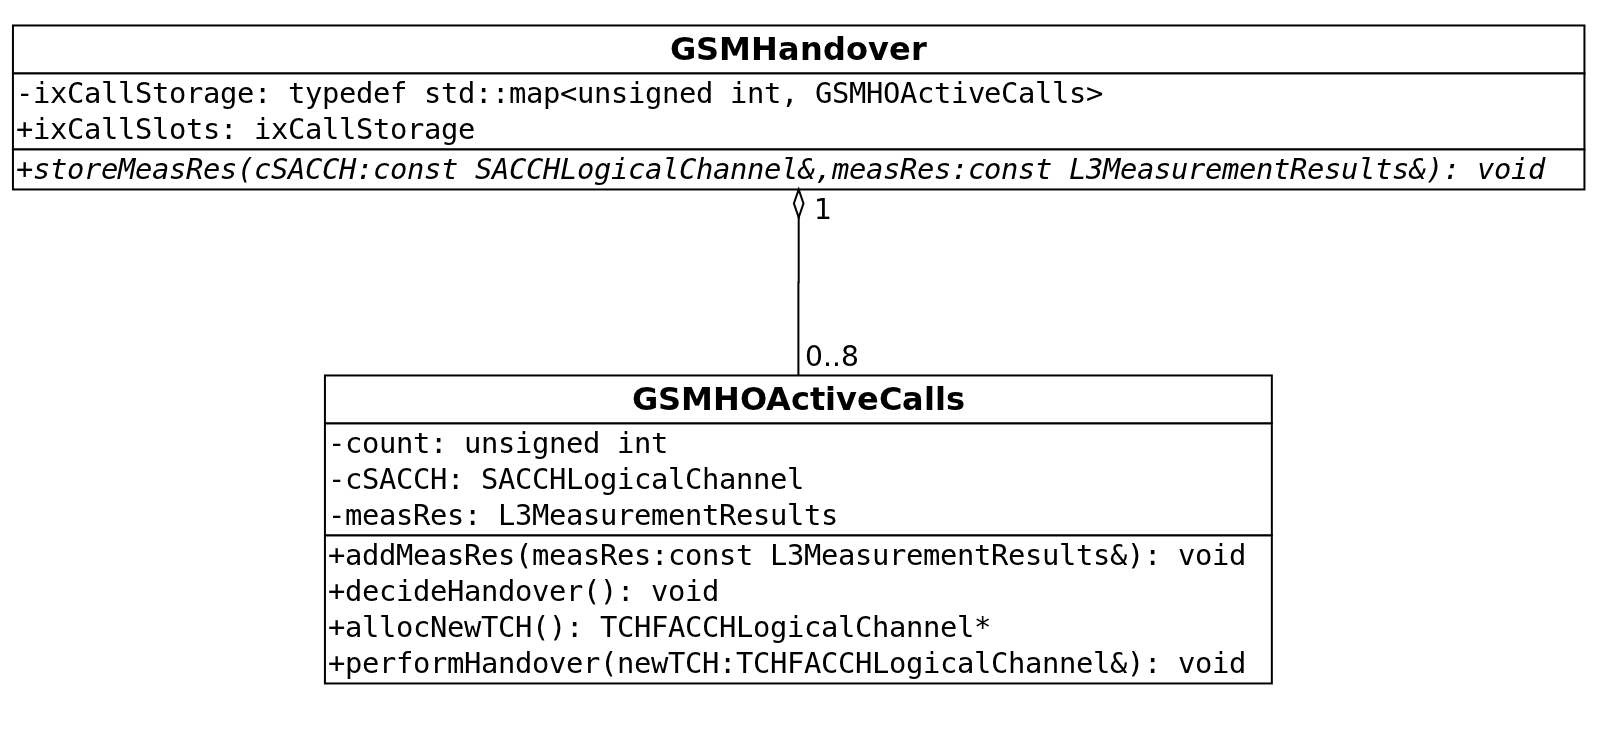
\includegraphics[width=0.8\textwidth]{img/homc}
  \caption{Klassendiagramm Handover-Modul}
  \label{fig:homclass}
\end{figure}

Von der Klasse \lstinline{GSMHandover} wir in der Datei \lstinline{OpenBTS.cpp} des \textit{apps}-Moduls ein globales Objekt instanziiert. Nach dem schreiben der aktuellen Measurement Reports in die SQLite3-Datenbank wird die Methode \lstinline{storeMeasRes()} des \lstinline{GSMHandover}-Objekts aufgerufen. Der Methode werden als Parameter die Referenz auf ein \lstinline{L3MeasurementResults}-Objekt und eine Referenz auf das entsprechende \lstinline{SACCHLogicalChannel}-Objekt übergeben. Mit Hilfe der Frequenz und des Timeslots des \gls{sacch} werden bis zu acht Objekte des Typs \lstinline{GSMHOActiveCalls} in der Map des \lstinline{GSMHandover}-Objekts verwaltet und die neusten Measurement Reports entsprechend zugeordnet.

Die Abarbeitung der restlichen in Abschnitt \ref{sec:handover} beschriebenen Aufgaben erfolgt mit Hilfe der Methoden der Klasse \lstinline{GSMHOActiveCalls}. Die Methode \lstinline{addMeasRes()} überschreibt dabei lediglich das in der Membervariablen gespeicherte Messergebnis. Hier wären zusätzliche Erweiterungen wie die speicherung von beispielsweise bis zu zehn Messergebnissen und die Bildung eines gleitenden Mittelwerts denkbar.

Die Methode \lstinline{decideHandover()} ist für die logische Entscheidungsfindung der Notwendigkeit eines Handover zuständig. In der aktuellen Implementierung prüft die Methode lediglich das vorhandensein der Datei \lstinline{doit} im aktuellen Arbeitsverzeichnis. Auf diese Art kann mit der Eingabe von \lstinline{touch doit} in einer Shell ein Handover manuell für Testzwecke ausgelöst werden. In Zukunft sollte diese Methode die Messergenisse von verscheidenen BTS berücksichtigen und eine logische Entscheidung treffen.

Für den Aufbau eines neuen TCH in einer benachbarten BTS ist eine Kommunikation zwischen den beiden System notwendig. Normalerweise erledigt diese Aufgabe der BSC. Im Fall von OpenBTS diese Kommunikation erst implementiert werden. Diese aufwändige Arbeit konnte im Rahmen der Projektarbeit allerdings nur theoretisch ausgearbeitet werden (siehe Abschnitt \ref{sec:interbts}). Aus diesem Grund wird in der Methode \lstinline{allocNewTCH()} ein TCH innerhalb des aktiven OpenBTS Systems geöffnet.

Der Methode \lstinline{performHandover()} wird als Parameter die Referenz auf den neu allozierten TCH übergeben. Anschließend wird das in Kapitel \ref{sec:swarch} beschriebene Handover-Command erzeugt und über den bestehenden FACCH an die Mobile Station gesendet. Das Umschalten der SIP-Verbindung wäre ein wichtiger Zwischenschritt, der in der aktuellen Implementierung nicht enthalten ist. Neben der Inter BTS Kommunikation, ist diese Aufgabe eine Ansatzpunkt für zukünftige Projektgruppen. Nachdem dem Senden des Handover-Command wir der alte TCH mit Hilfe der entsprechenden GSM-Primitive freigegeben.

Dieser Intra BTS Handover wurde in mehrer Tests erfolgreich durchgeführt und konnte bereits wie in Kapitel \ref{sec:analyse} beschrieben getraced und analysiert werden.
